\appendix
\renewcommand{\thesection}{\Alph{section}} % Nummerierung mit Buchstaben
\renewcommand{\thesubsection}{\thesection.\arabic{subsection}} % Zweite Ebene mit Zahlen
\renewcommand*{\sectionmark}[1]{\markright{Anhang \thesection: #1}}

\chapter{Anhang}
    
\section{Anleitung zur Verwendung} \label{subsec:anleitung_zur_verwendung}

Nach der korrekten Installation des Programms, welches in Kapitel \ref{sec:installation} beschrieben ist, kann das Programm wie folgt verwendet werden:
Die Installation ist zum Zeitpunkt der Übergabe dieser Arbeit bereits auf dem FESTO-PC erfolgt. 

Der Quellcode ist jederzeit unter folgender URL erreichbar: 
\url{https://github.com/andreasbraig/DHBWMA_HHAT_Image-Classification}

Im Branch main befindet sich die Version zum Zeitpunkt der Abgabe.

\textbf{Zunächst sollte auf folgende Punkte geachtet werden:}
\begin{itemize}
    \item Die Installation ist auf dem FESTO-PC erfolgt. Das Passwort ist bei Frau \BetreuerDHBW \ zu erfragen.
    \item Die verwendete Python Version ist 3.12.9.
    \item Alle verwendeten Bibliotheken sind in der requirements.txt Datei aufgelistet.
    \item Das Programmverzeichnis mit allen Daten liegt unter: 
    
    \texttt{D:/Repo/DHBWMA\_HHAT\_Image-Classification}
\end{itemize}


\textbf{Um das Programm auszuführen, bitte der folgenden Anleitung folgen:}

\begin{enumerate}
    \item Das PowerShell Skript auf dem Desktop mit dem Namen \texttt{Image\_classification.ps1} ausführen.
    \item Sobald in PowerShell die URL \texttt{http://127.0.0.1:5000} angezeigt wird, kann die Webseite im Browser geöffnet werden.
    \item Wenn mit der VISOR Kamera der FESTO \ac{cp-lab} Kamera Fotos archiviert werden, sollten diese auf der Website mit Klassifizierungsergebnis dargestellt werden. 
\end{enumerate}

Im Folgenden wird in zwei Methoden erklärt, wie Fotos mit der VISOR Kamera archiviert werden können:

\subsection{Manuelle Archivierung}

\begin{enumerate} 
    \item Die FESTO \ac{cp-lab} Anlage muss mit Strom und Druckluft versorgt sein.
    \item Auf dem FESTO-PC die Visor Software starten.
    \item Zunächst Config öffnen, das Passwort ist \texttt{Admin} für den Benutzer \texttt{admin}.
    \item Dieses Fenster kann direkt wieder geschlossen werden. (die Einstellungen sind bereits gespeichert, also \texttt{Yes} drücken)
    \item Im Visor Fenster auf \texttt{View} klicken und unten links \texttt{Archiving} durch Klicken aktivieren.
    \item Nun sollte die Kamera Fotos aufnehmen und diese in folgenden Ordner ablegen:
    
    \texttt{D:/Repo/DHBWMA\_HHAT\_Image-Classification/Bilder/new}

\end{enumerate}

\subsection{Automatische Archivierung}

Für diese Methode wurde in der \texttt{MES 4} Software der FESTO \ac{cp-lab} Anlage eine neue Order mit einem neuen Buffer erstellt, welcher den Job für die Kamera enthält. 

\begin{enumerate} 
    \item Die FESTO \ac{cp-lab} Anlage muss mit Strom und Druckluft versorgt sein.
    \item Die Software MES 4 auf dem FESTO-PC starten.
    \begin{figure}[H]
        \centering
        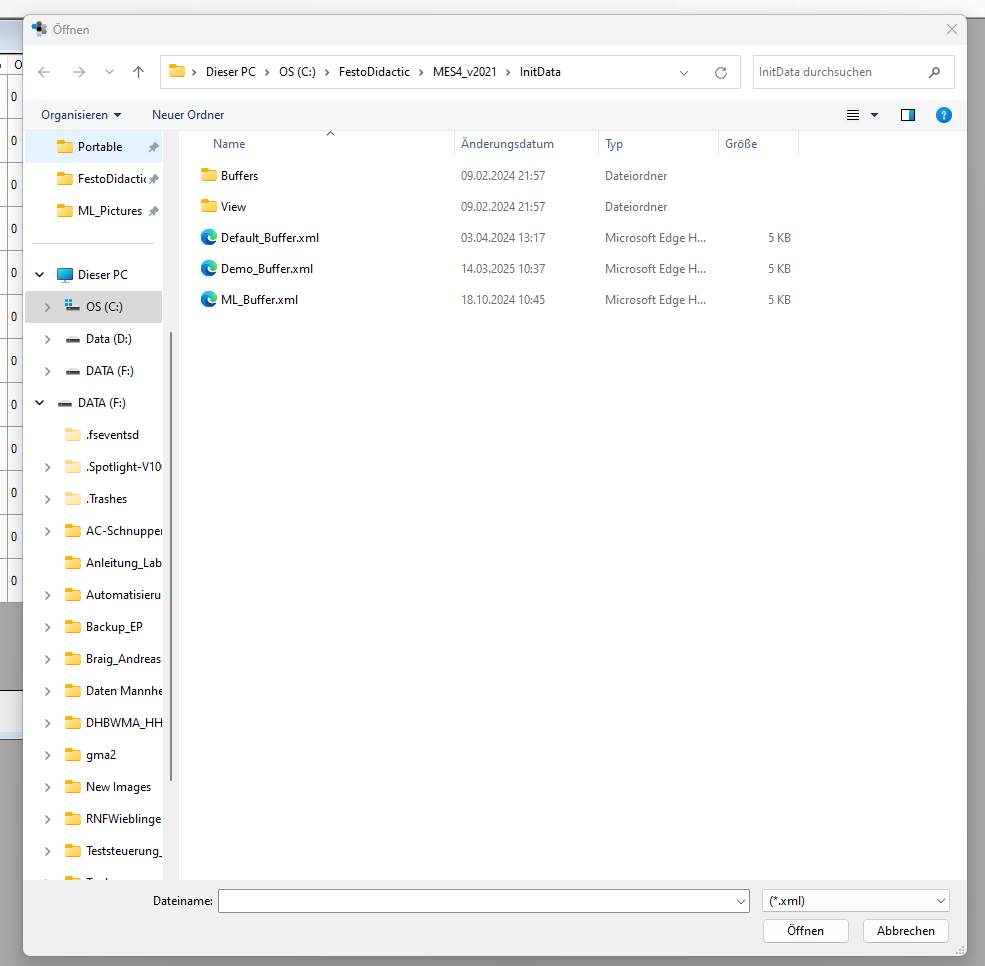
\includegraphics[width=0.7\textwidth]{Anleitung_Lab/Buffer_datei.png}
    \end{figure}
    \item In der MES 4 Software einen neuen Buffer laden, dieser ist mit dem Namen \texttt{Demo\_Buffer} versehen.
    \begin{figure}[H]
        \centering
        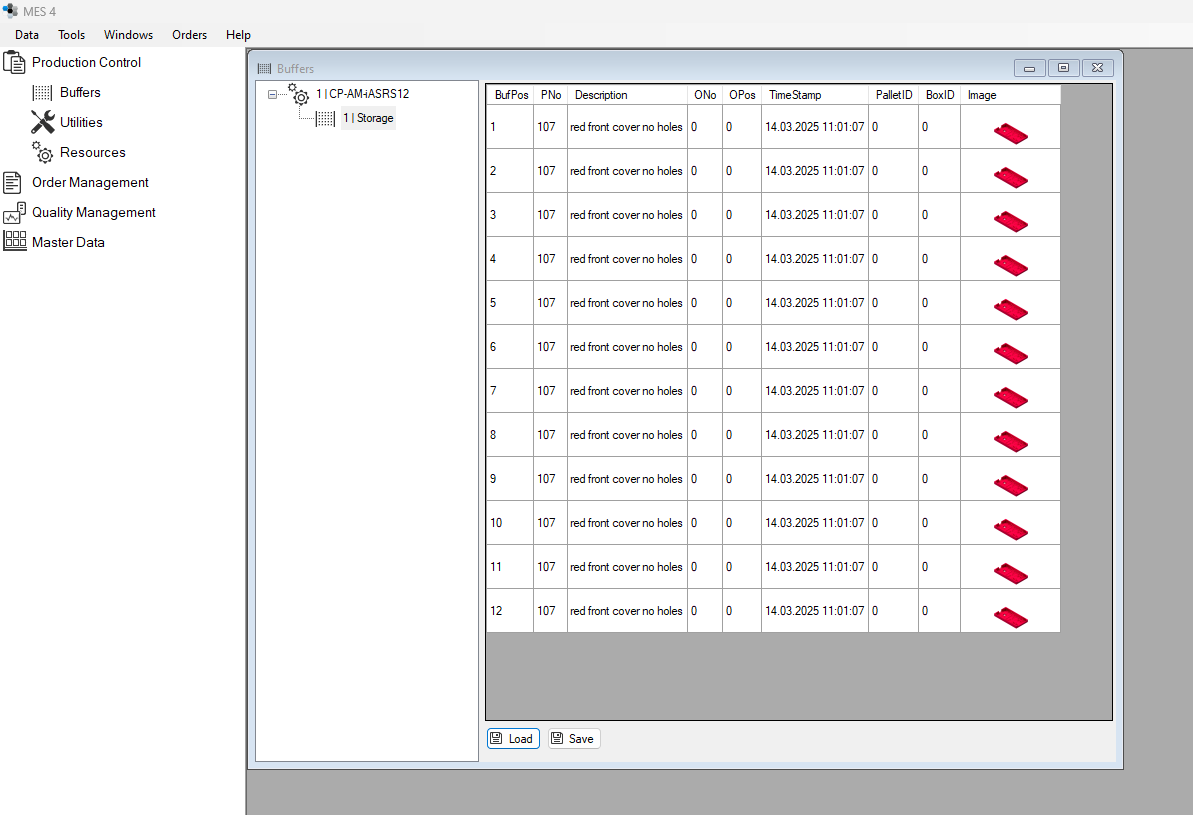
\includegraphics[width=0.7\textwidth]{Anleitung_Lab/Buffer_fertig.png}
    \end{figure}
    \item Der Buffer sollte jetzt mit pinken Boxen gefüllt sein.
    \item Über das \texttt{Planned Orders} Menü eine neue Order importieren. Diese liegt unter \texttt{C:/Users/Festo/Desktop/ML Pictures} ab.

    \begin{figure}[H]
        \centering
        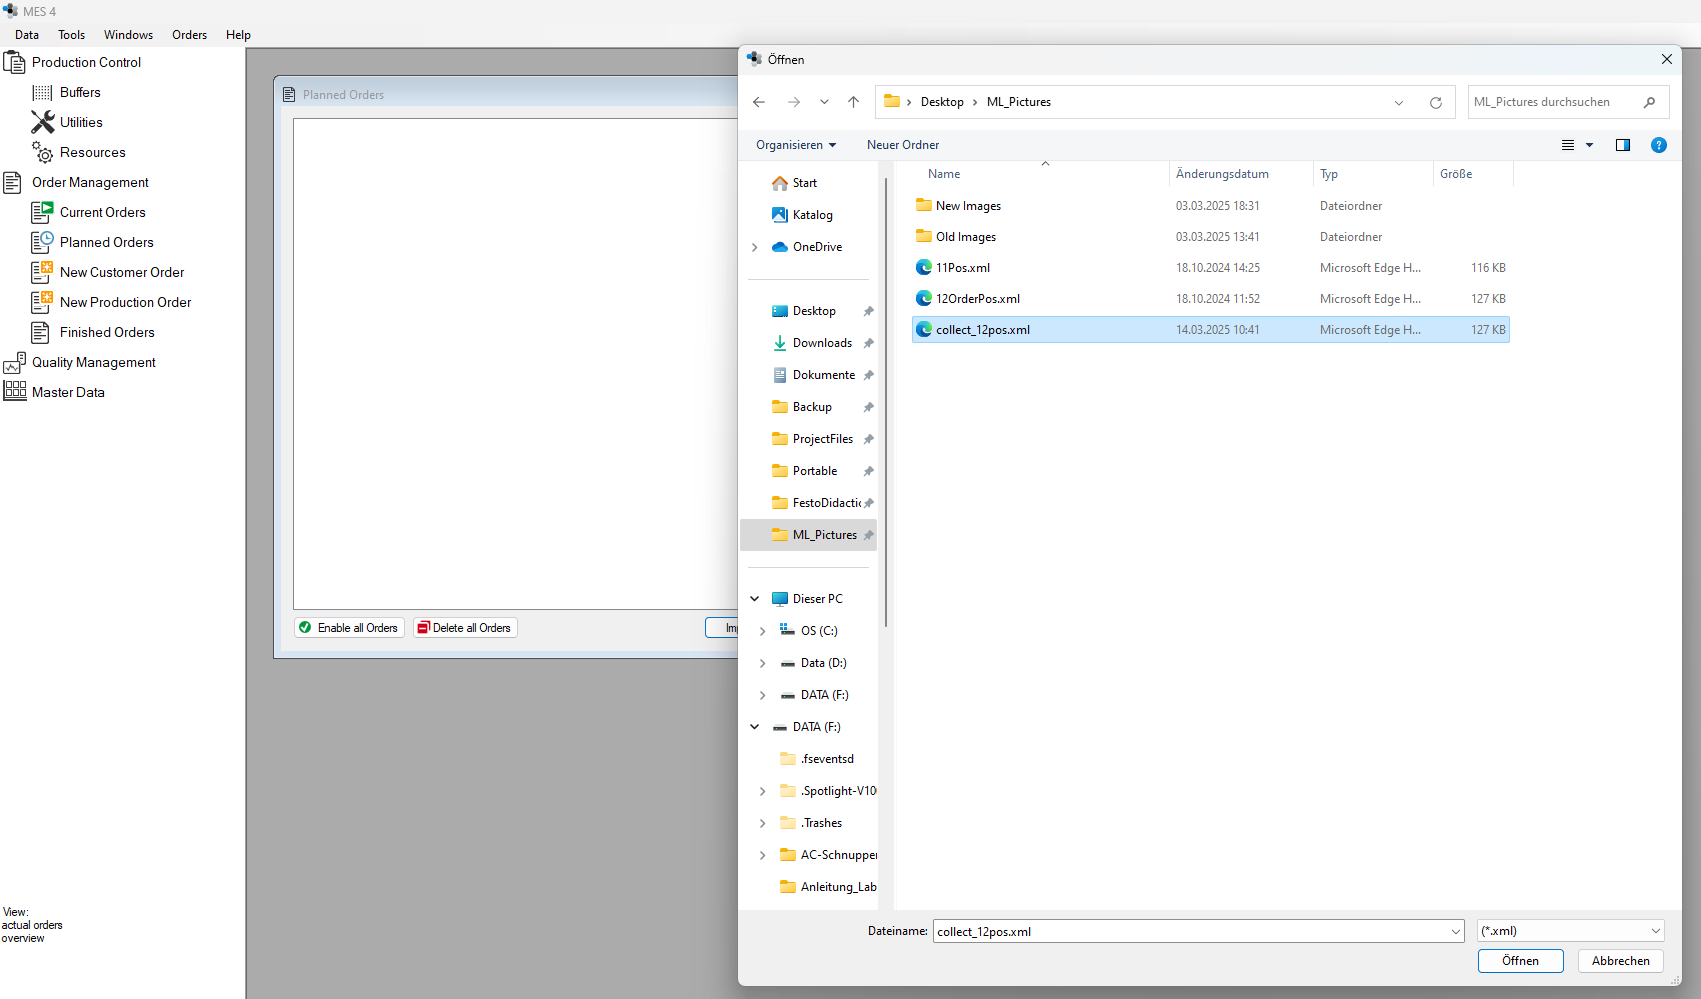
\includegraphics[width=0.7\textwidth]{Anleitung_Lab/Order.png}
    \end{figure}

    \item Die Order sollte jetzt in der MES 4 Software sichtbar sein und muss gestartet werden.
    \item Nun sollte die Kamera Fotos aufnehmen und diese in folgenden Ordner ablegen:
    
    \texttt{D:/Repo/DHBWMA\_HHAT\_Image-Classification/Bilder/new}

    \item Zur Kontrolle kann auf dem HMI der Kamerastation der aktuell ausgewählte Job betrachtet werden. Dieser sollte 7 sein.

\end{enumerate}

\section{Performance der Modelle} \label{sec:performance_der_modelle}

\subsection{Pytorch Custom CNN}

\begin{table}[H]
\centering
\begin{tabular}{|c|c|c|c|c|}
\hline
\multirow{2}{*}{\textbf{Label}} & \multicolumn{3}{c|}{\textbf{F1-Score}} & \textbf{Support} \\
\cline{2-4}
                               & \textbf{Precision} & \textbf{Recall} & \textbf{F1-Score} & \\
\hline
Bad                           & 1.00 & 0.96 & 0.98 & 47 \\
Good                          & 0.97 & 1.00 & 0.98 & 58 \\
\hline
\textbf{Accuracy}             & & & 0.98 & 105 \\
\hline
\textbf{Macro avg}            & 0.98 & 0.98 & 0.98 & 105 \\
\hline
\textbf{Weighted avg}         & 0.98 & 0.98 & 0.98 & 105 \\
\hline
\end{tabular}
\caption{Performance der Custom CNN (PyTorch) Modell}
\end{table}

\subsection{MobileNet V3 (TensorFlow)}

\begin{table}[H]
\centering
\begin{tabular}{|c|c|c|c|c|}
\hline
\multirow{2}{*}{\textbf{Label}} & \multicolumn{3}{c|}{\textbf{F1-Score}} & \textbf{Support} \\
\cline{2-4}
                               & \textbf{Precision} & \textbf{Recall} & \textbf{F1-Score} & \\
\hline
Bad                           & 0.44 & 1.00 & 0.61 & 46 \\
Good                          & 0.00 & 0.00 & 0.00 & 59 \\
\hline
\textbf{Accuracy}             & & & 0.44 & 105 \\
\hline
\textbf{Macro avg}            & 0.22 & 0.50 & 0.30 & 105 \\
\hline
\textbf{Weighted avg}         & 0.19 & 0.44 & 0.27 & 105 \\
\hline
\end{tabular}
\caption{Performance der MobileNet V3 (TensorFlow) Modell}
\end{table}

\subsection{MobileNet V1 (TensorFlow)}

\begin{table}[H]
\centering
\begin{tabular}{|c|c|c|c|c|}
\hline
\multirow{2}{*}{\textbf{Label}} & \multicolumn{3}{c|}{\textbf{F1-Score}} & \textbf{Support} \\
\cline{2-4}
                               & \textbf{Precision} & \textbf{Recall} & \textbf{F1-Score} & \\
\hline
Bad                           & 0.87 & 0.72 & 0.79 & 46 \\
Good                          & 0.81 & 0.92 & 0.86 & 59 \\
\hline
\textbf{Accuracy}             & & & 0.83 & 105 \\
\hline
\textbf{Macro avg}            & 0.84 & 0.82 & 0.82 & 105 \\
\hline
\textbf{Weighted avg}         & 0.83 & 0.83 & 0.83 & 105 \\
\hline
\end{tabular}
\caption{Performance der MobileNet V1 (TensorFlow) Modell}
\end{table}
